\renewcommand*{\arraystretch}{1.1}

\noindent\begin{tabularx}{\queryCardWidth}{|>{\queryPropertyCell}c|X|}
	\hline
	query & BI / 13 \\ \hline
%
	title & Popular Tags per month in a country \\ \hline
%
    pattern & \hfill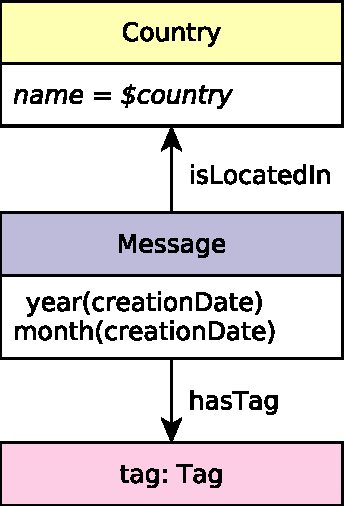
\includegraphics[scale=\patternscale,margin=0cm .2cm]{patterns/bi-read-13}\hfill\vadjust{} \\ \hline
%
	desc. & Find all Messages in a given Country, as well as their Tags.

For each group, find the 5 most popular Tags, where popularity is the
number of Messages (from within the same group) where the Tag appears.
 \\ \hline
%
	
        group by &
        \multicolumn{1}{>{\raggedright}X|}{
            \varName{year}, 
            \varName{month}
            } \\ \hline
	
%
	params &
	\innerCardVSpace{\begin{tabularx}{\attributeCardWidth}{|>{\paramNumberCell}c|>{\varNameCell}M|>{\typeCell}m{\typeWidth}|Y|} \hline
	\cellcolor{parameter} \color{white} \footnotesize $\mathsf{1}$ &country& String &  \\ \hline
	\end{tabularx}}\innerCardVSpace \\ \hline
%
	
        result &
        \innerCardVSpace{\begin{tabularx}{\attributeCardWidth}{|>{\resultNumberCell}c|>{\varNameCell}M|>{\typeCell}m{\typeWidth}|>{\resultOriginCell}c|Y|} \hline
        $\mathsf{1}$ & year & 32-bit Integer &C&
                year(message.creationDate) \\ \hline
        $\mathsf{2}$ & month & 32-bit Integer &C&
                month(message.creationDate) \\ \hline
        $\mathsf{3}$ & popularTags & TagPairs &C&
                (tag.name - String, popularity - 32-bit Integer), sorted descending by popularity, then ascending by tag name \\ \hline
        \end{tabularx}}\innerCardVSpace \\ \hline
	
%
	sort        &
        \innerCardVSpace{\begin{tabular}{|>{\sortNumberCell}c|>{\varNameCell}l|>{\directionCell}c|} \hline
        $\mathsf{1}$ & year & $\desc$ \\ \hline
        $\mathsf{2}$ & month & $\asc$ \\ \hline
        \end{tabular}}\innerCardVSpace \\ \hline
	%
	limit & 100 \\ \hline
	%
	CPs &
	\multicolumn{1}{>{\raggedright}l|}{
	    \chokePoint{1.2}, 
	    \chokePoint{2.2}, 
	    \chokePoint{2.3}, 
	    \chokePoint{3.2}, 
	    \chokePoint{6.1}
	    } \\ \hline
	%
    %
\end{tabularx}
\queryCardVSpace